\documentclass{article}
\usepackage[utf8]{inputenc}
\usepackage{graphicx} % Allows including images
\usepackage{subcaption}
\usepackage{amsmath}
\newcommand{\pluseq}{\mathrel{+}=}

\title{Weekly Report}
\author{Junior Team }
\date{August 2020}

\begin{document}

\maketitle

\section*{Introduction}
After presenting, we began to incorporate some of the ideas and feedback received from the group. We also began to prepare for out meeting with Nima scheduled next week. 

\section{Un-Normalized Error}
One common question in response to our different plots is are these trends simply due to normalization? For example, in figure \ref{fig:originalPlot}, it is possible that this trend is simply due to the amplification of errors due to the small denominators when in the normalization step. If we plot the un-normalized error however, we still see the same trend (Fig \ref{fig:newerPlot}), showing that this can't be due to normalization. 

\begin{figure}[h!]
    \centering
    \begin{subfigure}[b]{0.45\linewidth}
        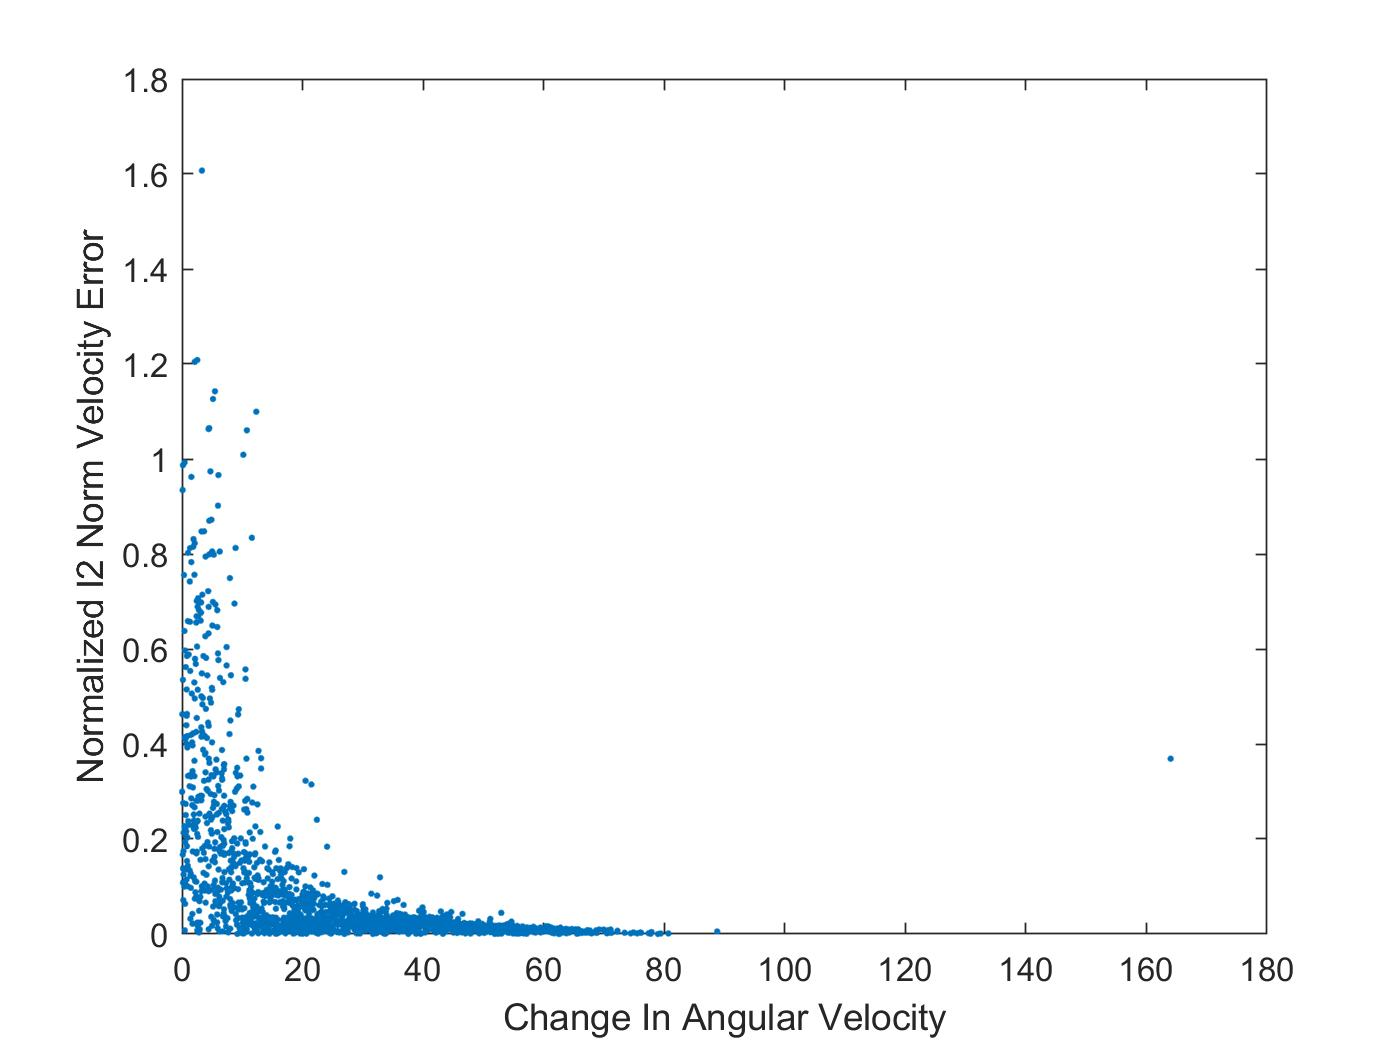
\includegraphics[scale=0.125]{changeInOmegaEllipse.jpg}
        \caption{Normalized Error}
        \label{fig:originalPlot}
    \end{subfigure}
    \quad
    \begin{subfigure}[b]{0.45\linewidth}
       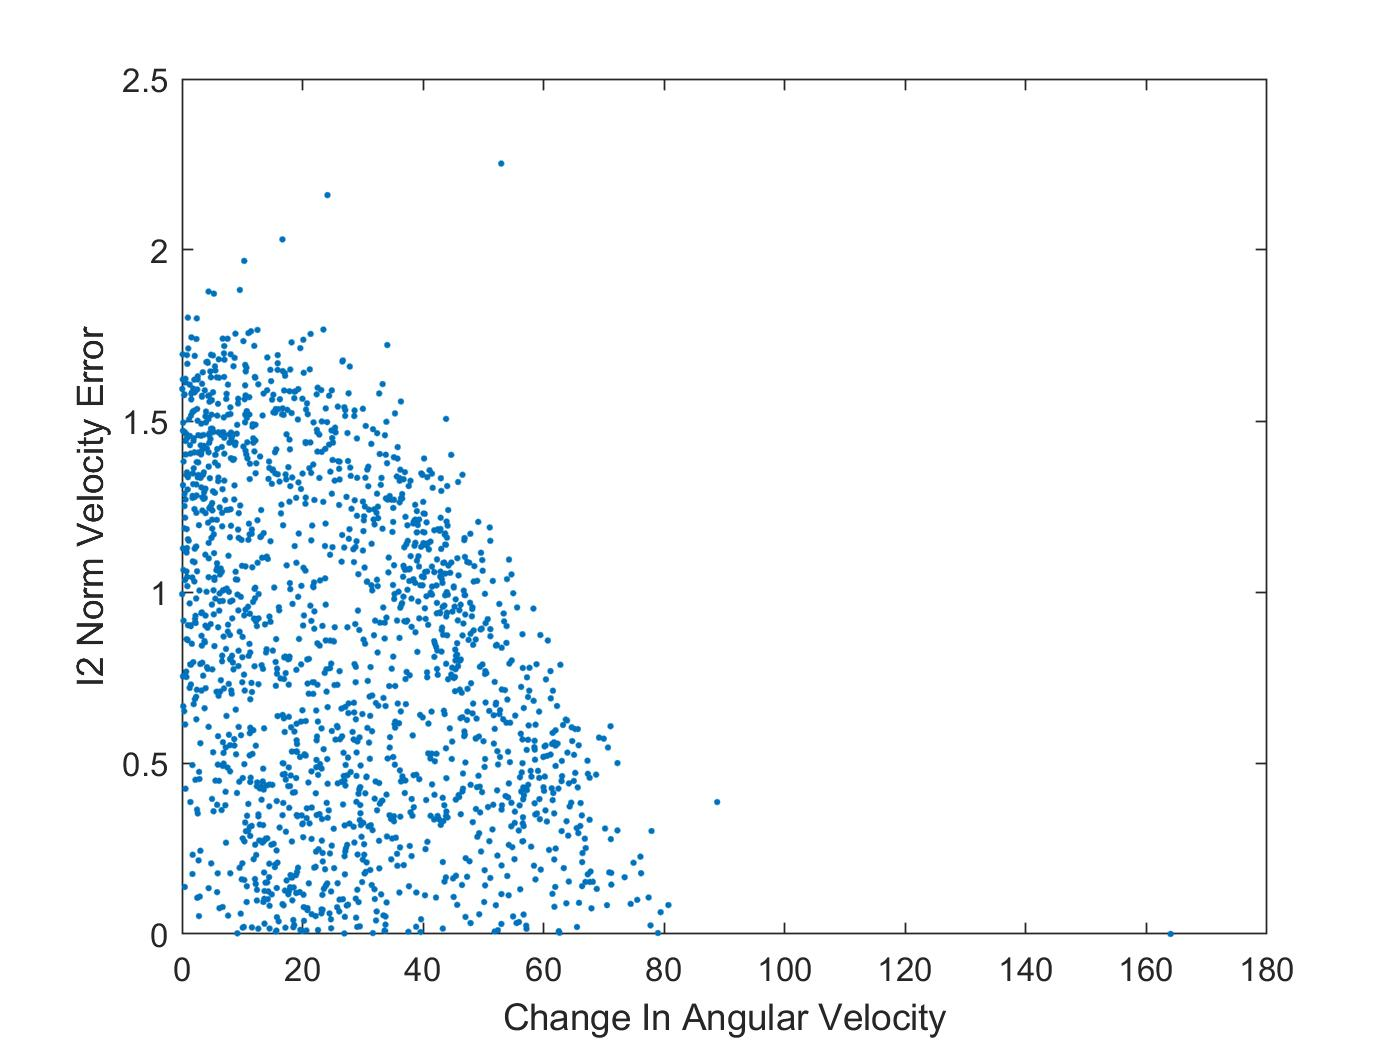
\includegraphics[scale=0.125]{newPlot.jpg}
        \caption{Ellipse Data Set}
        \label{fig:newerPlot}
    \end{subfigure}
    \caption{Examining the Effect of Normalization on this Trend}
\end{figure}


\noindent In addition to looking at the change in angular velocity, we can simply take the magnitude of post impact angular velocity and get the same trend (Fig. \ref{fig:3DPlot}). We see that usually if the impact leads to a lot of rotation, the IRB model has a better prediction than if it has low amounts of rotation after impact. Adding the total norm of Post impact velocity on the third axis further cements that this trend is not due to normalization. \\

\begin{figure}[h!]
    \centering
    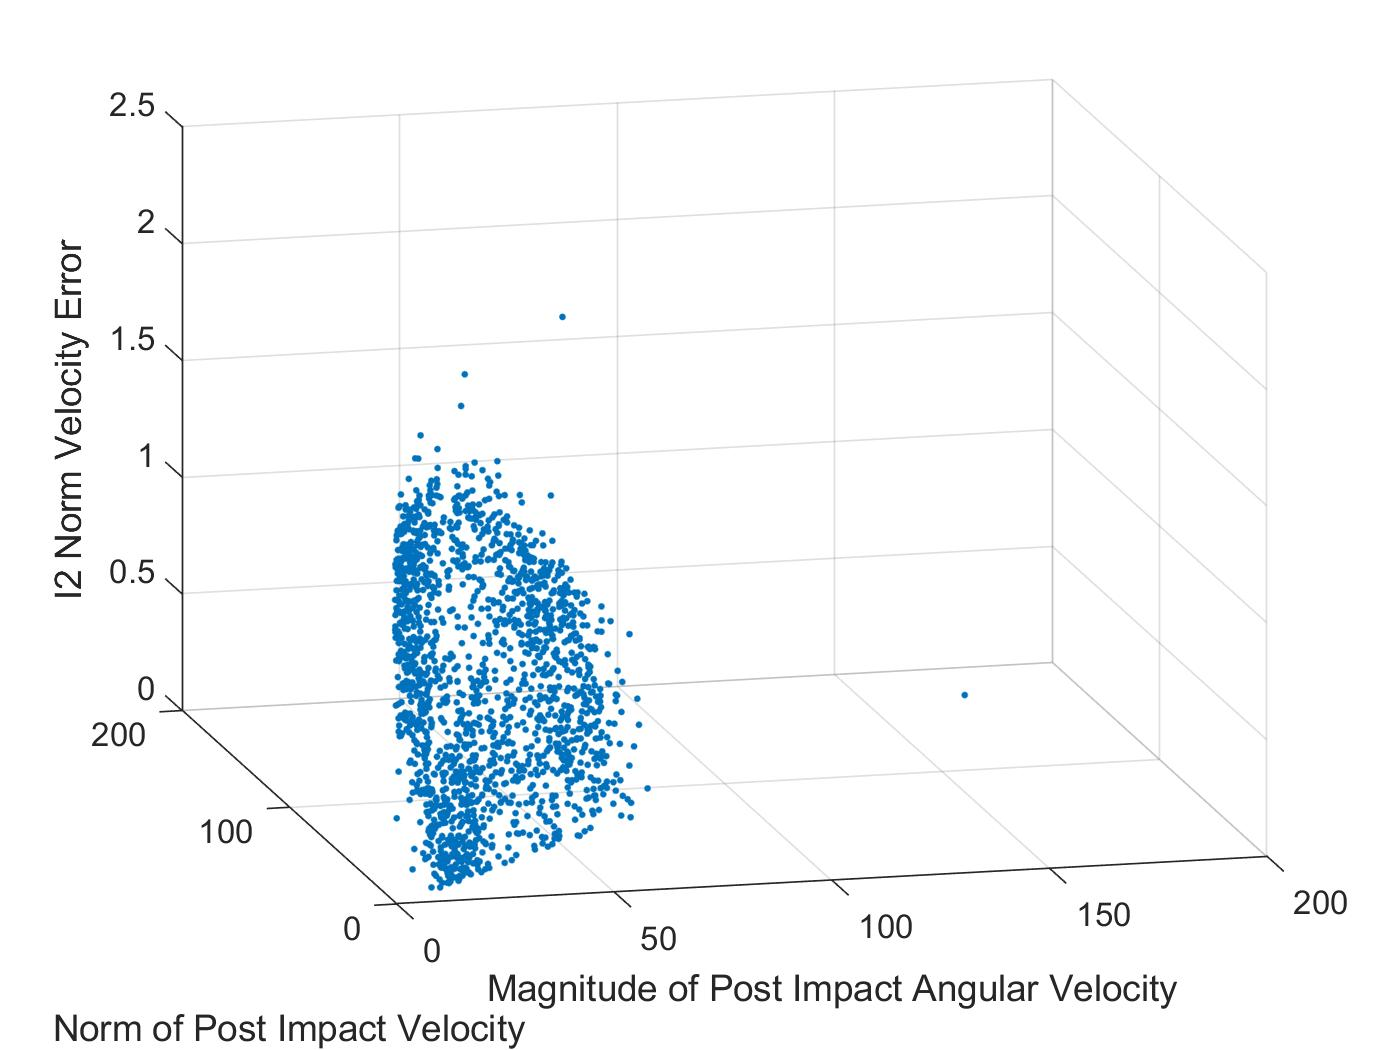
\includegraphics[scale = 0.25]{3DPlot.jpg}
    \caption{Investigating Error and Magnitude of Post Impact Angular Velocity}
    \label{fig:3DPlot}
\end{figure}

\noindent This is a rather counter intuitive finding, saying that when an object has a softer impact (lower velocity impact) and lower levels of rotations post impact, the IRB model tends to give worse predictions. Perhaps this can be explained by something mentioned later in the report or perhaps this is something that needs to be revisited starting with the fundamental physics of the problem. This trend is something we will continue to discuss and consider as we move forwards.

\newpage
\section{Improving Square Data Set}

\subsection{Removing Bad Data}
One nice benefit of plotting non-normalized error was the ability to spot data trials that had been marked as "good" but actually had issues like missing frames or a was double impact. After plotting all of the cases, we saved a list of all the trials that we above a certain error threshold and ran them all through the visualizer for manual inspection. Through this process, over twenty five impacts were eliminated and our total number of impacts in our data set was now a little under 300. This of course led to lower means for error in both the normalized and un-normalized cases.  

\subsection{Improving Velocity Fitting Methods}
As Matt pointed out in our presentation, the linear fitting method for extracting velocities should really be different for the y case. Since the object is in free fall, we do not expect the position curve to be linear, but rather to follow a parabolic trajectory. To factor this in, we subtracted the effect of gravity on the position, then performed a linear fit. The method can be explained via this series of steps:

\begin{align*}
    \mbox{Position Vector: } y = [y_0,\ y_1,\ ...,\ y_n] \\
    \mbox{Time Vector: } t = [t_0,\ t_1,\ ...,\ t_n] \\
    \mbox{Filter Position Vector:  } y_* = y +\frac{1}{2}g(t-t_0)^2 \\
    \mbox{Apply a  Linear Fit: } polyfit(t, y_*),\ y_* = mt+ b \\
    \mbox{Rewrite Position Vector: } y = mt + b - \frac{1}{2}g(t-t_0)^2 \\
    \mbox{Calculate Velocity: } v(t_n)  = m - g (t_n - t_0) 
\end{align*}



\subsection{Improving Jacobian Calculations}
After our presentation, we were hearing a lot of suggestions with respect to the way we involve angular velocity. The idea of including the angular velocity component when calculating our contact Jacobian was something we found interesting, so we decided to focus some of our time on that. As we mentioned before, we were calculating the contact Jacobian as shown: 

\begin{equation}
n = 
\begin{bmatrix} 
 0 \\
 1 \\
 x_{COM}-x_{contact} 
\end{bmatrix}
\end{equation}

\begin{equation}
d = 
\begin{bmatrix} 
 1 \\
 0 \\
 y_{COM}-y_{contact} 
\end{bmatrix}
\end{equation}

\noindent However, we wanted to improve the accuracy of these calculations by including angular velocity when detecting/simulating an impact. The way we did this was by first examining when the y-velocity of the square changed signs from negative to positive. Initially, we would then take the data from a frame before to begin simulating the square's trajectory with minuscule time steps ($\Delta t = 10^{-7}  s$), but we were finding that going back only one frame gave us inconclusive results. We found that making our beginning frame (time $t = 0$) two frames back would yield conclusive solutions within our specified tolerance. We began at time $t = 0$ and iterated through, simulating the square's trajectory and positioning with the following assumptions: 

% \begin{align*}
%     \mbox{Constant x Velocity : } x = \dot{x} t + x_0 \\ 
%     \mbox{Constant y Acceleration (Freefall) : }  y = \frac{-1}{2} gt^{2} + \dot{y} t + y_0 \\
%     \mbox{Constant y Acceleration (Freefall) : } \dot{y} = -gt + \dot{y_0} 
    
% \end{align*}
  
\begin{equation}
    \mbox{Constant x velocity: } x = \dot{x} t + x_0  
\end{equation}
\begin{equation}
    \mbox{Constant Angular Velocity : } \theta = \omega t + \theta_0
\end{equation}
\begin{equation}
     \mbox{Freefall: }y = \frac{-1}{2} gt^{2} + \dot{y} t + y_0 
\end{equation}
\begin{equation}
    \mbox{Freefall: }\dot{y} = -gt + \dot{y_0} 
\end{equation}



\end{document}
